\section{Physics}
                          \begin{multicols}{2}

                            \fmSubSec{Dinámica}
                            \begin{itemform}
                            \item Peso
                              $$w=mg$$
                            \item 2da Ley de Newton:
                              $$\vec{F} = m\vec{a} \quad \magn{N} = \magn{kg\cdot \dfrac{m}{s^2}}$$
                            \item Fuerza centrípeta:
                              $$F_c = m\frac{v^2}{r} \quad \magn{N}$$
                            \item Momento lineal:
                              $$\vec{p} = m\vec{v} \quad \magn{kg\cdot \dfrac{m}{s}}$$
                            \end{itemform}
                            \fmSubSec{MRU}
                            Considerandose
                            $$F=ma=mg \rightarrow a=g\rightarrow v$$
                            integrando sobre tiempo
                            \begin{multicols}{2}                                
                            \begin{itemform}
                            \item Velocidad
                              $$v=gt+v_0$$
                            
                            \columnbreak
                            \item Posicion
                              $$x=\dfrac{gt^2}{2}+v_0t+x_0$$
                            \end{itemform}
                            \end{multicols}

                            \fmSubSec{Caida Libre}
                            Para caida libre se considera $x_0=0$ y $v_0=0$

                            \begin{itemform}
                            \item Velocidad
                              $$\evalat{v=gt+v_0}{v_0=0}\Rightarrow\boxed{v = gt}$$
                              $$
                              y = \frac{g}{2} \cdot \left(\frac{v}{g}\right)^2 = \frac{v^2}{2g} \Rightarrow \boxed{v^2 = 2gy}
                              $$

                            \item Posicion
                              $$y = \dfrac{gt^2}{2} + v_0 t + s_0\Rightarrow \boxed{y=\dfrac{gt^2}{2}}$$

                            \end{itemform}

                            \fmSubSec{Tiro Vertical}
                            Para tiro vertical se considera la aceleración negativa y $h_{max}=0$
                            \begin{itemform}
                            \item Tiempo en $h_max$
                              $$0 = v_0 - gt \Rightarrow t = \frac{v_0}{g}$$
                            \item  Altura (Considerandose el tiempo obtenido)
                              $$h = v_0 \cdot \frac{v_0}{g} - \frac{g}{2} \cdot \left( \frac{v_0}{g} \right)^2
                              = \frac{v_0^2}{g} - \frac{v_0^2}{2g} = \boxed{h = \frac{v_0^2}{2g}}$$
                            \item Formula energetica
                              $$  v^2 = v_0^2 - 2g h \Rightarrow \boxed{v^2 = v_0^2 - 2gh}$$

                            \end{itemform}
                            \fmSubSec{Cinemática}
                            Se considera $\theta=s/r$ siendo s segmento de arco y r radio, Ademas que $a=\sqrt{a_T^2+a_c^2}$, mientras que el periodo se define $T=\dfrac{2\pi}{\omega}$
                            \subsubsection*{Angular}
                            \begin{itemform}
                            \item Velocidad angular:
                              $$\vec{\omega} = \frac{d\theta}{dt} \quad \magn{\dfrac{rad}{s}}$$
                            \item Aceleración centrípeta:
                              $$a_c = \frac{v^2}{r} = \omega^2 r \quad \magn{\dfrac{m}{s^2}}$$
                            \end{itemform}
                            Para cinematica se aplican las mismas formulas que MRU cambiando $v\to\omega\quad  x\to \theta$
                            $$\omega_f = \omega_0 \pm \alpha t \quad
                            \theta = \omega_0 t \pm \dfrac{\alpha t^2}{2} \quad
                            \omega_f^2 = \omega_0^2 \pm 2\alpha\theta
                            $$
                            \subsubsection*{Tangencial}
                            Se considera la velocidad como $v=\omega R$ y se consideran las mismas formulas que MRU, $a\to a_T=aR$

                            $$v_f = v_0 \pm a_T t \quad
                            L = v_0 t \pm \dfrac{a_T t^2}{2} \quad
                            v_f^2 = v_0^2 \pm 2a_T L$$


                            \fmSubSec{Rotaciones}
                            \begin{itemform}
                            \item Torque:
                              $$\vec{\tau} = \vec{r}\times\vec{F} \quad \magn{N\cdot m} \quad \tau=Fd\sin \theta$$
                            \item Momento de inercia:
                              $$I = \sum m_i r_i^2 \quad \magn{kg\cdot m^2}$$
                            \item Energía cinética rotacional:
                              $$K_{\text{rot}} = \frac{1}{2}I\omega^2 \quad \magn{J}$$

                            \end{itemform}

                            \fmSubSec{Energía y Trabajo}
                            \begin{multicols}{3}
                                \begin{itemform}
                            \item W mecánico:
                              $$W = \int \vec{F}\cdot d\vec{r} \quad \magn{J}$$
                            \item Teorema trabajo-energía:
                              $$\Delta K = W_{\text{neto}}$$
                            \item Energía Cinética:
                              $$K=\dfrac{1}{2}mv^2$$

                                \end{itemform}
                            \end{multicols}
                            \begin{itemform}
                            \item Potencia instantánea:
                              $$P = \frac{dW}{dt} = \vec{F}\cdot\vec{v} \quad \magn{W}$$
                            \item Potencia Eléctrica
                              $$\dfrac{d}{dt}(U=Q\Delta V) \rightarrow P=\dfrac{dQ}{dt}\Delta V  \rightarrow P=I\Delta V \quad \magn{W}$$
                            \end{itemform}

                            \end{multicols}

                            
                            \fmSubSec{Capacitores y Configuraciones}
                            \begin{itemform}
                            \item \textbf{Definición básica}:
                              $$ C = \dfrac{Q}{\Delta V} \quad \magn{F} $$

                            \item \textbf{Campo eléctrico (placas paralelas)}:
                              $$ E = \dfrac{\sigma}{\epsilon_0} = \dfrac{Q}{\epsilon_0 A} $$

                            \item \textbf{Energía almacenada}:
                              $$ U = \dfrac{1}{2}CV^2 = \dfrac{1}{2}QV = \dfrac{Q^2}{2C} $$

                            \item \textbf{Carga en función del tiempo (descarga)}:
                              $$ Q(t) = Q_0 e^{-t/RC} $$
                            \end{itemform}
                            \fmSubSec{Configuraciones de Capacitores}
                            \begin{multicols}{2}

                              \begin{itemform}

                              \item \textbf{Placas paralelas}:
                                $$ C = \dfrac{\epsilon_0 \epsilon_r A}{d} $$

                              \item \textbf{Esférico}:
                                $$ C = \dfrac{4\pi\epsilon_0}{\dfrac{1}{a} - \dfrac{1}{b}} $$

                              \item \textbf{Cilíndrico}:
                                $$ C = \dfrac{2\pi\epsilon_0 L}{\ln(b/a)} $$

                              \item \textbf{En serie}:
                                $$ C_{eq} = \left(\sum_{i=1}^n \dfrac{1}{C_i}\right)^{-1} $$

                              \item \textbf{En paralelo}:
                                $$ C_{eq} = \sum_{i=1}^n C_i $$

                              \end{itemform}
                              
                          \end{multicols}
              
                    \newpage
    \section{Electricidad y Magnetismo}
    \begin{multicols}{2}
             \begin{itemize}[leftmargin=*]
                              \item $e = 1.6\times10^{-19}\ \magn{C} \quad k = \dfrac{1}{4\pi\epsilon_0} \approx 9\times10^9\ \magn{\dfrac{N\cdot m^2}{C^2}}$
                              \item $1\ \text{T} = 10^4\ \text{G (Gauss)} \quad \magn{T}=\magn{\dfrac{Wb}{m^2}}=\magn{\dfrac{\frac{J}{A}}{m^2}}=\magn{\dfrac{N}{Am}}$

                              \item $\epsilon_0 = 8.85\times10^{-12}\ \magn{\dfrac{C^2}{N\cdot m^2}} \mu_0 = 4\pi\times10^{-7}\ \magn{\dfrac{T\cdot m}{A}}$
                              \item $m_e = 9.11\times10^{-31}\ \magn{kg} \quad m_p = 1.7\times10^{-27}\ \magn{kg}$
                              
                                           \item Torque magnético y Momento dipolar:
                              $$\vec{\tau} = \vec{\mu}\times\vec{B} \quad \magn{N\cdot m} \qquad \vec{\mu} = I\vec{A} \quad \magn{A\cdot m^2}$$
   \columnbreak
                              \item                             Fuerza de Lorentz:
                            $$\vec{F} = q\vec{v}\times\vec{B} +q\vec{E}\quad \magn{N}$$
    \item Densidad Campo
    $$\vec{D}=\epsilon_0 \vec{E} \magn{\dfrac{C}{m^2}} \quad \vec{B}=\mu_0 \vec{H} \magn{\dfrac{Wb}{m^2}}$$

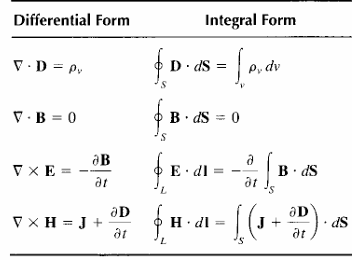
\includegraphics[width=0.61\linewidth]{src/MaxwelLaws.png}

    \end{itemize}
    \end{multicols}
    
    
\begin{multicols}{2}
\vspace{-0.5pt}
  \fmSubSec{Electricidad}

  \subsubsection*{Leyes Clave}
  \begin{itemize}[leftmargin=*]
      \item Ley de Faraday:
    $$\oint \vec{E}\cdot d\vec{l} = -\frac{d\Psi_B}{dt} \quad \magn{V}$$

  \end{itemize}

  \subsubsection*{Fenómenos Eléctricos}
  \begin{itemform}
    \item Ley de Coulomb:
    $$\vec{F} = k\frac{|q_1q_2|}{r^2}\hat{r} \quad \magn{N}$$
    \item Ley de Gauss \textbf{I Maxwell}: 
    $$\Phi=\oint \vec{E}\cdot d\vec{S} = \frac{Q_{\text{enc}}}{\epsilon_0} \quad \oint \vec{D}\cdot d\vec{S} = Q_{\text{enc}} \  \magn{\dfrac{N\cdot m^2}{C}}$$
    \item Campo eléctrico:
    $$\vec{E} = k\frac{q}{r^2}\hat{r} \quad \vec{E}=-\nabla V  \magn{\dfrac{N}{C}}  \magn{\dfrac{V}{m}}$$
  \end{itemform}

  \subsubsection*{Energía y Potencial}
  \begin{itemform}
    \item Diferencia de potencial \textbf{III Maxwell}:
    $$\Delta V = -\int \vec{E}\cdot d\vec{l}  \quad \magn{V} \quad \oint \vec{E}\cdot d\vec{l}=0$$
%    \item Energía potencial:
 %   $$U = k\frac{q_1q_2}{r} \quad \magn{J} \quad W=q \Delta V$$
    \item Densidad de carga:
    $$\lambda = q/L \text{  } \magn{\dfrac{C}{m}} \quad
    \sigma = q/A \text{  }\magn{\dfrac{C}{m^2}} \quad
    \rho = q/V \text{  }\magn{\dfrac{C}{m^3}}$$
  \end{itemform}

  \subsection*{Potenciales}
  \begin{multicols}{2}
      
  \begin{itemform}
    \item \textbf{Carga puntual:}
    $$V=k\dfrac{q}{r}$$
    \item \textbf{en una linea:}
    $$\Delta V = Ed$$
    \item \textbf{Cilindro:}
    $$\Delta V= \dfrac{\lambda}{2 \pi r \epsilon_0}$$
    \item \textbf{Dipolo:}
    $$V=\dfrac{2a|q|k \cos \theta}{r^2}$$
  \end{itemform}
  \end{multicols}

\columnbreak
  \fmSubSec{Magnetismo}

  \subsubsection*{Leyes Clave}
  \begin{itemize}[leftmargin=*]
    \item Ley de Ampère \textbf{IV Maxwell}:
    $$\dfrac{\oint \vec{B}\cdot d\vec{l}}{\mu_0} = \oint \vec{H}\cdot d\vec{l} = \int \vec{J} \cdot d\vec{S} =  I_{\text{enc}} \quad \magn{A}$$
  \end{itemize}

  \subsubsection*{Fenómenos Magnéticos}
  \begin{itemform}
    \item Fuerza Magnética ($dq\vec{U}=Id\vec{l}$):
    $$\vec{F_B}= \oint_{L} Id\vec{l}\times\vec{B}=\oint_{S} (\vec{K}ds)\times\vec{B}=\oint_{S} (\vec{J}dv)\times\vec{B}$$
    \item Flujo Magnético \textbf{II Maxwell}:
    $$\Psi_B = \int_S \vec{B}\cdot d\vec{A}=\int \vec{A} \cdot d\vec{l}  \quad \magn{Wb} \quad \oint_S \vec{B}\cdot d\vec{A}=0$$
    \item Biot-Savart:
    $$d\vec{B}=\dfrac{\mu_0I}{4\pi}\dfrac{d\vec{l}\times\hat{r}}{r^2} \magn{\dfrac{Wb}{m^2}}\quad d\vec{H}=\dfrac{I}{4\pi}\dfrac{d\vec{l}\times\hat{r}}{r^2} \magn{\dfrac{A}{m}}$$
    \item Fuerza por unidad de longitud:
    $$\frac{F}{L} = \frac{\mu_0 I_1I_2}{2\pi d} \quad \magn{\dfrac{N}{m}}$$
  \end{itemform}

  \subsection*{Campos Magnéticos}
  \begin{itemform}
    \item \textbf{Alambre finito:}
    $$\vec{H}=\dfrac{1}{4 \pi} \dfrac{I}{\rho} (\cos(\alpha_2)-\cos(\alpha_1)) \ \hat{a_\phi}$$
    \item \textbf{Alambre semi infinito y semi-finito:}
    $$\vec{H}=\dfrac{1}{4 \pi} \dfrac{I}{\rho}  \ \hat{a_\phi} \qquad \vec{H}=\dfrac{1}{2 \pi} \dfrac{I}{\rho}  \ \hat{a_\phi}$$

  \end{itemform}
\end{multicols}

  \newpage
\begin{multicols}{2}
\fmSubSec{Orita le pongo nombre perron}
\begin{itemform}

% -------------------------------
% CABLE COAXIAL
% -------------------------------
\item \textbf{Cable Coaxial}
\[
H_{\phi}=
\begin{cases}
\dfrac{I\rho}{2\pi a^2} & 0 \le \rho \le a\\[6pt]
\dfrac{I}{2\pi\rho} & a \le \rho \le b\\[6pt]
\dfrac{I}{2\pi\rho}\left[1-\dfrac{\rho^2-b^2}{t^2+2bt}\right] & b \le \rho \le b+t\\[6pt]
0 & \rho \ge b+t
\end{cases}
\]

% -------------------------------
% PLANOS INFINITOS
% -------------------------------
\item \textbf{Planos Infinitos}
\[
\vec{H}=\dfrac{1}{2}(\vec{K}\times\hat{n}), \qquad 
\vec{B}=\dfrac{1}{2}\mu_0(\vec{K}\times\hat{n})
\]

% -------------------------------
% LÁMINA DE CORRIENTE
% -------------------------------
\item \textbf{Lámina de Corriente}
\[
\mathbf{H} =
\begin{cases}
-\dfrac{K}{2}\,\mathbf{a}_x & z>z_0\\[4pt]
+\dfrac{K}{2}\,\mathbf{a}_x & z<z_0
\end{cases}
\]

% -------------------------------
% POTENCIAL VECTORIAL
% -------------------------------
\end{itemform}
\textbf{Potenciales}
\begin{itemform}
    
\item \textbf{Potencial Magnético Vectorial } $\vec{A} \magn{\dfrac{Wb}{m}}$ 
$$
\vec{A}
=\int_{\text{lin}} \frac{\mu}{4\pi}\frac{I\,d\vec{l}}{R}
=\int_{\text{sup}} \frac{\mu}{4\pi}\frac{\vec{K}\,dS}{R}
=\int_{\text{vol}} \frac{\mu}{4\pi}\frac{\vec{J}\,dv}{R}
$$
\item \textbf{Potencial Magnetico Vectorial}
$$
\nabla \cdot \vec{A}=0
$$

$$
\vec{B}=\nabla\times\vec{A}
$$


% -------------------------------
% POTENCIAL ESCALAR MAGNÉTICO
% -------------------------------
\item \textbf{Potencial Magnético Escalar} $V_m$ Si ($\vec{J}=0$)
\[
\vec{H}=-\nabla V_m
\]
Ecuación de Poisson ($\vec{J}=0$): 
\[
\nabla^2 V_m = 0
\]
% -------------------------------
% ECUACIÓN PARA A (POISSON)
% -------------------------------
\item \textbf{Laplaciano del Potencial Vectorial}
\[
\nabla^2 \vec{A} = -\mu_0 \vec{J}
\]

\item \textbf{Ley Faraday (Fuerza Electromotriz)}
$$
V_{emf}=-\dfrac{d\lambda}{dt}=-N \dfrac{d\Psi}{dt}
$$
$$
V_{emf}= \oint\vec{E} \cdot d\vec{l}= -\dfrac{d}{dt} \int_S \vec{B} \cdot d\vec{S}
$$

$$
V_{emf}= - \int_S \dfrac{\partial B }{\partial t}\cdot d\vec{S} +\oint_L (\vec{u} \times \vec{B}) \cdot d\vec{l}
$$

\item  Ley Faraday Bara recta
$$
V_{emf}=uBL \sin \theta
$$
\item Ley Faraday Espira
$$
V_{emf}=NBAw \sin \theta
$$

\end{itemform}
\textbf{Corrientes}
\begin{itemform}
    \item Carga 
    $$Q=\int_S \vec{D} \cdot d\vec{S}$$
    \item \textbf{Corriente de Convección}
    $$
    I=\rho_v \Delta S \dfrac{\Delta l}{\Delta t}=\rho_v \Delta S  u_y \quad I=\int \vec{J} \cdot d\vec{S}
    $$
    \item \textbf{Densidad de Corriente de conduccion}
    $$J=\dfrac{\Delta I}{\Delta S}=\sigma E \quad \vec{J}=\rho_v \vec{u}$$
    \item \textbf{Densidad de Corriente de Desplazamiento}
    $$\textbf{J}_d=\dfrac{\partial \textbf{D}}{dt}$$
    \item \textbf{Ecuación Continuidad}
$$
\vec{\nabla} \cdot \vec{J}+\dfrac{\partial\rho_v}{\partial t}=0
$$

\end{itemform}
\end{multicols}

\newpage
\section{Mecánica Lagrangiana y Hamiltoniana}
\begin{multicols}{2}

\fmSubSec{Mecánica Lagrangiana}

\subsubsection*{Fundamentos}
\begin{itemform}
\item Lagrangiano:
$$\mathcal{L} = T - V \quad \magn{J}$$

\item Ecuaciones de Euler-Lagrange:
$$\frac{d}{dt}\left(\frac{\partial \mathcal{L}}{\partial \dot{q}_i}\right) - \frac{\partial \mathcal{L}}{\partial q_i} = 0$$

\item Momento generalizado:
$$p_i = \frac{\partial \mathcal{L}}{\partial \dot{q}_i} \quad \magn{kg\cdot\dfrac{m}{s}}$$

\item Fuerza generalizada:
$$Q_i = \frac{\partial \mathcal{L}}{\partial q_i} \quad \magn{N}$$

\item Con fuerzas no conservativas:
$$\frac{d}{dt}\left(\frac{\partial \mathcal{L}}{\partial \dot{q}_i}\right) - \frac{\partial \mathcal{L}}{\partial q_i} = Q_i^{\text{nc}}$$
\end{itemform}

\subsubsection*{Sistemas Particulares}

\begin{itemform}
\item \textbf{Partícula libre:}
$$\mathcal{L} = \frac{1}{2}m\dot{x}^2 \Rightarrow p = m\dot{x}$$

\item \textbf{Partícula en campo gravitatorio:}
$$\mathcal{L} = \frac{1}{2}m(\dot{x}^2 + \dot{y}^2) - mgy$$

\item \textbf{Oscilador armónico:}
$$\mathcal{L} = \frac{1}{2}m\dot{x}^2 - \frac{1}{2}kx^2$$

\item \textbf{Péndulo simple:}
$$\mathcal{L} = \frac{1}{2}mL^2\dot{\theta}^2 + mgL\cos\theta$$

\item \textbf{Partícula en campo E-M:}
$$\mathcal{L} = \frac{1}{2}m\vec{v}^2 - q\phi + q\vec{A}\cdot\vec{v}$$
\end{itemform}

\subsubsection*{Coordenadas Generalizadas}

\begin{itemform}
\item \textbf{Coordenadas cilíndricas:}
$$T = \frac{1}{2}m(\dot{\rho}^2 + \rho^2\dot{\phi}^2 + \dot{z}^2)$$

\item \textbf{Coordenadas esféricas:}
$$T = \frac{1}{2}m(\dot{r}^2 + r^2\dot{\theta}^2 + r^2\sin^2\theta\,\dot{\phi}^2)$$

\item \textbf{Momento angular (coord. cíclica):}

Si $\frac{\partial \mathcal{L}}{\partial \phi} = 0 \Rightarrow p_\phi = \text{const}$
\end{itemform}

\columnbreak

\fmSubSec{Mecánica Hamiltoniana}

\subsubsection*{Fundamentos}
\begin{itemform}
\item Hamiltoniano:
$$\mathcal{H} = \sum_i p_i\dot{q}_i - \mathcal{L} = T + V \quad \magn{J}$$

\item Ecuaciones de Hamilton:
$$\dot{q}_i = \frac{\partial \mathcal{H}}{\partial p_i} \qquad \dot{p}_i = -\frac{\partial \mathcal{H}}{\partial q_i}$$

\item Corchetes de Poisson:
$$\{f,g\} = \sum_i \left(\frac{\partial f}{\partial q_i}\frac{\partial g}{\partial p_i} - \frac{\partial f}{\partial p_i}\frac{\partial g}{\partial q_i}\right)$$

\item Evolución temporal:
$$\frac{df}{dt} = \{f,\mathcal{H}\} + \frac{\partial f}{\partial t}$$

\item Transformación canónica ($\mathcal{H}'=\mathcal{H}+\frac{\partial F}{\partial t}$):
$$p_i = \frac{\partial F}{\partial q_i} \qquad P_i = -\frac{\partial F}{\partial Q_i}$$
\end{itemform}

\subsubsection*{Sistemas Particulares}

\begin{itemform}
\item \textbf{Partícula libre:}
$$\mathcal{H} = \frac{p^2}{2m}$$

\item \textbf{Oscilador armónico:}
$$\mathcal{H} = \frac{p^2}{2m} + \frac{1}{2}kx^2$$

\item \textbf{Partícula en potencial central:}
$$\mathcal{H} = \frac{p_r^2}{2m} + \frac{p_\theta^2}{2mr^2} + V(r)$$

\item \textbf{Rotador rígido:}
$$\mathcal{H} = \frac{p_\theta^2}{2I} + \frac{p_\phi^2}{2I\sin^2\theta}$$
\end{itemform}


\fmSubSec{Aplicaciones a Sistemas Físicos}

\begin{itemform}
\item \textbf{Péndulo doble:}
$$\mathcal{L} = \frac{1}{2}(m_1+m_2)L_1^2\dot{\theta}_1^2 + \frac{1}{2}m_2L_2^2\dot{\theta}_2^2$$
$$+ m_2L_1L_2\dot{\theta}_1\dot{\theta}_2\cos(\theta_1-\theta_2)$$
$$+ (m_1+m_2)gL_1\cos\theta_1 + m_2gL_2\cos\theta_2$$

\item \textbf{Partícula cargada en campo B:}
$$\mathcal{H} = \frac{1}{2m}(\vec{p}-q\vec{A})^2 + q\phi$$

\item \textbf{Problema de Kepler:}
$$\mathcal{H} = \frac{p_r^2}{2m} + \frac{L^2}{2mr^2} - \frac{k}{r}$$
donde $L = p_\phi = mr^2\dot{\phi}$ es conservado

\item \textbf{Relación con Newton:}
$$\vec{F} = m\vec{a} \Leftrightarrow \dot{p}_i = -\frac{\partial V}{\partial q_i}$$
\end{itemform}

\end{multicols}

\newpage
\section{Ondas Electromagnéticas}
\begin{multicols}{2}


\fmSubSec{Ecuación de Onda}

\begin{itemform}
\item \textbf{Para los campos Eléctricos y magnéticos}:
$$\nabla^2 \vec{E} - \mu_0\epsilon_0\frac{\partial^2 \vec{E}}{\partial t^2} = 0$$
$$\nabla^2 \vec{B} - \mu_0\epsilon_0\frac{\partial^2 \vec{B}}{\partial t^2} = 0$$

\item \textbf{Velocidad de la luz en el vacío}:
$$c = \frac{1}{\sqrt{\mu_0\epsilon_0}} \approx 3 \times 10^8 \quad \magn{\frac{m}{s}}$$

\item \textbf{En un medio}:
$$v = \frac{c}{n} = \frac{1}{\sqrt{\mu\epsilon}} \quad n = \sqrt{\mu_r\epsilon_r}$$
donde $n$ es el índice de refracción
\end{itemform}

\fmSubSec{Ondas Planas}


\begin{itemform}
\item \textbf{Forma general}:
$$\vec{E}(\vec{r},t) = \vec{E}_0 e^{i(\vec{k}\cdot\vec{r} - \omega t)} \quad \vec{B}(\vec{r},t) = \vec{B}_0 e^{i(\vec{k}\cdot\vec{r} - \omega t)}$$

\item \textbf{Número de onda}:
$$k = \frac{\omega}{v} = \frac{2\pi}{\lambda} \quad \magn{\frac{rad}{m}}$$

\item \textbf{Relación de dispersión}:
$$\omega = vk = \frac{ck}{n}$$

\item \textbf{Relación entre campos}:
$$|\vec{B}| = \frac{|\vec{E}|}{v} = \frac{n|\vec{E}|}{c} \quad \vec{E} \perp \vec{B} \perp \vec{k}$$
\end{itemform}


\fmSubSec{Vector de Poynting y Energía}

\begin{itemform}
\item \textbf{Vector de Poynting}:
$$\vec{S} = \frac{1}{\mu_0}\vec{E} \times \vec{B} = \frac{1}{\mu}\vec{E} \times \vec{H} \quad \magn{\frac{W}{m^2}}$$

\item \textbf{Intensidad (promedio temporal)}:
$$I = \langle S \rangle = \frac{1}{2}\sqrt{\frac{\epsilon_0}{\mu_0}}E_0^2 = \frac{cB_0^2}{2\mu_0} \quad \magn{\frac{W}{m^2}}$$

\item \textbf{Densidad de energía electromagnética}:
$$u = u_E + u_B = \frac{1}{2}\epsilon_0 E^2 + \frac{1}{2\mu_0}B^2 \quad \magn{\frac{J}{m^3}}$$

\item \textbf{Para ondas planas}:
$$u_E = u_B \quad u = \epsilon_0 E^2 = \frac{B^2}{\mu_0}$$

\item \textbf{Relación intensidad-densidad}:
$$I = uc \quad S = u v$$
\end{itemform}
\columnbreak
\begin{figure}
	\centering
	\includegraphics[width=0.5\linewidth]{src/FM3_Physics-11-01-25.png}
	\caption{figure}
	\label{fig:placeholder}
\end{figure}
\fmSubSec{Presión de Radiación}

\begin{multicols}{2}
\begin{itemform}
\item \textbf{Absorción total}:
$$P_{\text{rad}} = \frac{I}{c} = \frac{\langle S \rangle}{c} \quad \magn{Pa}$$

\columnbreak
\item \textbf{Reflexión total}:
$$P_{\text{rad}} = \frac{2I}{c} = \frac{2\langle S \rangle}{c} \quad \magn{Pa}$$
\end{itemform}
\end{multicols}

\begin{itemform}
\item \textbf{Momento lineal de un fotón}:
$$p = \frac{E}{c} = \frac{h\nu}{c} = \frac{h}{\lambda} = \hbar k$$
\end{itemform}

\fmSubSec{Reflexión y Refracción}

\begin{multicols}{2}
\begin{itemform}
\item \textbf{Ley de Snell}:
$$n_1\sin\theta_1 = n_2\sin\theta_2$$

\columnbreak
\item \textbf{Ángulo crítico}:
$$\sin\theta_c = \frac{n_2}{n_1} \quad (n_1 > n_2)$$
\end{itemform}
\end{multicols}

\begin{itemform}
\item \textbf{Coeficientes de Fresnel (incidencia normal)}:
$$r = \frac{n_1 - n_2}{n_1 + n_2} \quad t = \frac{2n_1}{n_1 + n_2}$$

\item \textbf{Reflectancia y Transmitancia}:
$$R = |r|^2 = \left(\frac{n_1-n_2}{n_1+n_2}\right)^2 \quad T = \frac{n_2}{n_1}|t|^2 = \frac{4n_1n_2}{(n_1+n_2)^2}$$
$$R + T = 1$$

\item \textbf{Ángulo de Brewster (polarización)}:
$$\tan\theta_B = \frac{n_2}{n_1}$$
\end{itemform}

\fmSubSec{Polarización}

\begin{itemform}
\item \textbf{Ley de Malus}:
$$I = I_0\cos^2\theta$$

\item \textbf{Polarización lineal}:
$$\vec{E} = E_0(\cos\phi\,\hat{x} + \sin\phi\,\hat{y})e^{i(kz-\omega t)}$$

\item \textbf{Polarización circular}:
$$\vec{E} = \frac{E_0}{\sqrt{2}}(\hat{x} \pm i\hat{y})e^{i(kz-\omega t)}$$

\item \textbf{Polarización elíptica (general)}:
$$E_x = E_{0x}\cos(kz-\omega t) \quad E_y = E_{0y}\cos(kz-\omega t + \delta)$$
\end{itemform}

\fmSubSec{Espectro Electromagnético}

\begin{itemize}[leftmargin=*,noitemsep,topsep=0pt]
\item \textbf{Ondas de radio}: $\lambda > 1$ m, $f < 300$ MHz
\item \textbf{Microondas}: $1$ mm $< \lambda < 1$ m
\item \textbf{Infrarrojo}: $700$ nm $< \lambda < 1$ mm
\item \textbf{Visible}: $400$ nm $< \lambda < 700$ nm
\item \textbf{Ultravioleta}: $10$ nm $< \lambda < 400$ nm
\item \textbf{Rayos X}: $0.01$ nm $< \lambda < 10$ nm
\item \textbf{Rayos Gamma}: $\lambda < 0.01$ nm
\end{itemize}

\vspace{0.3cm}
\textbf{Relación frecuencia-longitud de onda:}
$$c = \lambda f \quad E = h\nu = \frac{hc}{\lambda}$$
donde $h = 6.626 \times 10^{-34}$ J·s (constante de Planck)

\end{multicols}
